\documentclass[journal]{IEEEtran}
\usepackage{cite}
\usepackage{amsmath,amssymb}
\usepackage{graphicx}
\usepackage{booktabs}
\usepackage{xcolor}
\usepackage{url}
\usepackage{textcomp}
\usepackage[colorlinks=true,allcolors=blue]{hyperref}

\definecolor{accessblue}{RGB}{0,114,172}
\newcommand{\todo}[1]{\textcolor{red}{[TODO: #1]}}
% PINN coordinate scheme is not yet signed off (CLAUDE.md Sec. 2); flag every PINN number.
\newcommand{\pinn}{$^{\dagger}$}

\begin{document}

\title{\textcolor{accessblue}{\Large\bfseries Fetal Cardiac Ageing Clock: A Multi-Cohort Framework for Non-Invasive Fetal ECG Extraction and Cardiac Maturity Estimation}}

\author{\IEEEauthorblockN{BHUVANESH S., CHANDRAPRAKASH K., TEJA SREE C., AND MUTHUKUMAR K. A.}
\IEEEauthorblockA{Department of Computer Science and Engineering, SSN College of Engineering, Chennai, India\\
Corresponding author: Muthukumar K. A. (\todo{email})}
\thanks{\todo{funding / acknowledgement statement}}}

\markboth{Bhuvanesh S.\ et al.: Fetal Cardiac Ageing Clock}{}
\maketitle

\begin{abstract}
We present a multi-cohort pipeline that starts from noisy multi-channel maternal abdominal ECG, extracts a fetal ECG, computes 12 interpretable cardiac biomarkers, and regresses a Cardiac Age (CA) whose difference from the LMP-dated gestational age (GA), $\Delta\mathrm{Age}=\mathrm{CA}-\mathrm{GA}$, is proposed as a candidate IUGR screening index. Extraction combines multivariate EMD (MEMD) artefact removal, adaptive maternal-ECG cancellation, a physics-informed neural network (PINN) with a Laplace constraint, and a FastICA blind-source-separation (BSS) fallback chosen per window by a quality gate. On the CinC 2013 cohort, never trained on, the hybrid extractor reaches a QRS F1 of 0.542 (PINN alone 0.377); on NInFEA, scored against pulsed-wave Doppler, it recovers a heart rate within 10~bpm of the reference in 54\% of windows (PINN alone 2\%) and raises the number of usable recordings from 3 to 55 of 60. A contrastive VAE and a transformer then estimate CA. This part does \emph{not} yet work: within NInFEA (GA 21--27 weeks) neither the Doppler fetal heart rate nor any of the 12 biomarkers correlates significantly with GA, and strict leave-one-mother-out MAE (22.6~d) is worse than predicting the cohort mean (12.5~d). We report this negative result and its causes, and list what data and decisions are needed before the ageing claim can be tested.
\end{abstract}

\begin{IEEEkeywords}
Fetal ECG, non-invasive fetal monitoring, multivariate empirical mode decomposition, physics-informed neural network, contrastive variational autoencoder, gestational age estimation, intrauterine growth restriction.
\end{IEEEkeywords}

\section{Introduction}
\IEEEPARstart{I}{ntrauterine} growth restriction (IUGR), most commonly caused by placental insufficiency that develops silently, is reported to cause over one million neonatal deaths annually, with roughly 30\% of cases undetected until delivery~\todo{cite source for these statistics}. Ultrasound biometry captures structural growth only and cardiotocography (CTG) captures acute distress only; neither quantifies the \emph{functional} maturation of the fetal heart. The fetal ECG (fECG) recorded from the maternal abdomen is an attractive but hard signal source: the fetal component is a few microvolts, buried under the maternal ECG (mECG), baseline drift, motion and muscle artefact, and mains interference. If the fECG could be extracted reliably, quantities derived from it (heart-rate variability, ventricular repolarisation, depolarisation morphology) might track fetal cardiac maturity. A model that maps such quantities to a ``Cardiac Age'' (CA) would give $\Delta\mathrm{Age}=\mathrm{CA}-\mathrm{GA}$, a continuous deviation of cardiac maturity from the dated gestational age.

Prior work from our group used a 1D-CNN with EMD-based quality gating for fECG extraction~\cite{muthukumar2026icc}; Wahbah et al.\ reported 94.2\% (subject-dependent) and 88.8\% (subject-independent) fetal R-peak detection accuracy with a BiLSTM~\cite{wahbah2024}. Such results show that automated fetal cardiac signal analysis is feasible, but a model that performs well within one dataset does not necessarily generalise to other populations, hardware or gestational windows, and extraction-only studies do not estimate fetal cardiac age. Both~\cite{muthukumar2026icc,wahbah2024} are also trained to regress a scalp or R-peak reference, which exists in only one public dataset. We instead ask whether a pipeline that combines signal-processing priors, a physics constraint and blind source separation can transfer to cohorts that have no amplitude reference, and whether features computed from its output carry gestational-age information.

The contributions and, equally important, the limits of this paper are:
\begin{enumerate}
\item A complete, reproducible pipeline (preprocessing, MEMD, maternal cancellation, PINN, FastICA, quality gate, 12 biomarkers, contrastive VAE, transformer, leave-one-subject-out evaluation) over three public cohorts.
\item A hybrid extractor that uses the PINN output only when it passes a quality gate and falls back to FastICA otherwise. It is the best extractor on all three cohorts, and it is evaluated against Doppler timing on NInFEA, a reference we derived from the dataset's Doppler bitmaps.
\item A documented negative result: the 12 biomarkers show no detectable age signal within NInFEA, and the age model does not beat a predict-the-mean baseline. We analyse why.
\end{enumerate}

The rest of the paper is organised as follows. Section~II reviews related work, Section~III describes the datasets, Section~IV states the problem and the method, Section~V the experimental protocol, Section~VI the results, Section~VII discusses limitations and Section~VIII concludes.

\section{Related Work}
Table~\ref{tab:related} summarises the studies closest to this work.

\begin{table*}[!t]
\caption{Summary of related work.}
\label{tab:related}
\centering
\small
\begin{tabular}{@{}p{3.0cm}p{6.8cm}p{6.8cm}@{}}
\toprule
Study & Method and key finding & Limitation \\
\midrule
Wahbah et al.\ (2024)~\cite{wahbah2024} & BiLSTM fetal ECG extraction from abdominal ECG; 94.2\% accuracy (subject-dependent), 88.8\% (subject-independent) & Extraction and R-peak detection only; no cardiac-age estimation; no broad cross-dataset evaluation \\
Motie-Shirazi et al.\ (2025)~\cite{motie2025} & Self-supervised gestational-age estimation from low-cost Doppler ultrasound & Doppler rather than ECG; does not use fetal ECG morphology \\
Gu et al.\ (2025)~\cite{gu2025} & CTG-derived ``cardiotocography age'' as a biomarker for adverse pregnancy outcomes & CTG rather than ECG; no analysis of fetal cardiac electrical characteristics \\
Hoyer et al.\ (2013)~\cite{hoyer2013} & Fetal functional brain age from heart-rate and autonomic patterns & Targets brain maturation, not cardiac maturity from ECG \\
\bottomrule
\end{tabular}
\end{table*}

ECG-based age and health estimation has also been studied on adult datasets such as PTB-XL~\cite{ptbxl} and MIMIC-IV-ECG~\cite{mimicecg}. Their outcome is disease classification on adult recordings, whereas ours is fetal cardiac-maturity regression; their populations, acquisition and signal characteristics differ, and they do not require maternal--fetal source separation.

Table~\ref{tab:existing} contrasts the common practice with the proposed system. Prior work separately addresses fECG extraction (timing accuracy) or age-like biomarkers from other modalities (Doppler, CTG); cardiac-maturation estimation from the fetal ECG across independent cohorts has not been demonstrated.

\begin{table}[!t]
\caption{Existing approaches versus the proposed system.}
\label{tab:existing}
\centering
\small
\begin{tabular}{@{}p{1.6cm}p{2.9cm}p{3.2cm}@{}}
\toprule
 & Existing & Proposed \\
\midrule
Extraction & Adaptive filtering / ICA, tuned per dataset & MEMD + cancellation + PINN, FastICA fallback \\
Reference & One reference type per study & Dataset-matched (scalp ECG / Doppler / expert QRS) \\
Output & Fetal heartbeat / QRS & Cardiac age and $\Delta$Age \\
Transfer & Rarely beyond training set & Three cohorts \\
Validation & Point-estimate accuracy & LOSOCV, bootstrap CI, baselines \\
\bottomrule
\end{tabular}
\end{table}

\section{Datasets}
Table~\ref{tab:data} summarises the cohorts. All internal quantities use 4 abdominal channels at 1000~Hz; GA and CA are stored in days.

\begin{table}[!t]
\caption{Cohorts used. $^{*}$GA of ADFECGDB records is known only as a 38--41 week range (see Section~VII).}
\label{tab:data}
\centering
\small
\begin{tabular}{@{}lccc@{}}
\toprule
 & ADFECGDB & NInFEA & CinC 2013 \\
\midrule
Records & 5 & 60 (39 mothers) & 25 (set-a) \\
Native rate & 1 kHz & 2048 Hz & 1 kHz \\
Abdominal ch. & 4 & 24 & 4 \\
Reference & scalp ECG & Doppler & fetal QRS \\
GA & 38--41 wk$^{*}$ & 21--27 wk & not published \\
Role & train & train/CV & zero-shot \\
\bottomrule
\end{tabular}
\end{table}

\textbf{ADFECGDB}~\cite{adfecgdb,goldberger2000}: five 5-minute recordings with a direct scalp lead (\texttt{Direct\_1}) used only as ground truth, never as model input. \textbf{NInFEA}~\cite{sulas2021}: 60 recordings with 24 abdominal unipolar channels plus non-physiological channels (\texttt{dc1--dc4}, \texttt{saw}, \texttt{sync}) and synchronised pulsed-wave Doppler, which provides fetal beat timing but no amplitude reference. \textbf{CinC 2013}~\cite{silva2013}: 25 one-minute records of 4 abdominal channels with fetal QRS annotations only.

Note the GA coverage gap: the training cohort spans 38--41 weeks, NInFEA 21--27 weeks, and nothing covers 28--37 weeks.

\section{Problem Formulation and Method}
\subsection{Problem formulation}
The abdominal recording is modelled as
\begin{equation}
X(t)=M(t)+F(t)+N(t),
\end{equation}
where $M$ is the maternal ECG (5--50$\times$ stronger than the fetal signal), $F$ the fetal ECG and $N$ noise and artefact. The pipeline must estimate $\widehat F\approx F$, compute a 12-dimensional feature vector, map it through a latent code to a cardiac age $\widehat{CA}$, and report
\begin{equation}
\Delta\mathrm{Age}=\widehat{CA}-GA,
\end{equation}
where $GA$ is the LMP-dated gestational age, an external label that is never a model input or output. Train and test subjects are disjoint, $S_{\mathrm{train}}\cap S_{\mathrm{test}}=\emptyset$. $\Delta$Age is analysed as a developmental deviation measure, not as an independently clinically validated label.

Fig.~\ref{fig:arch} gives the overall architecture.
\begin{figure*}[!t]
\centering
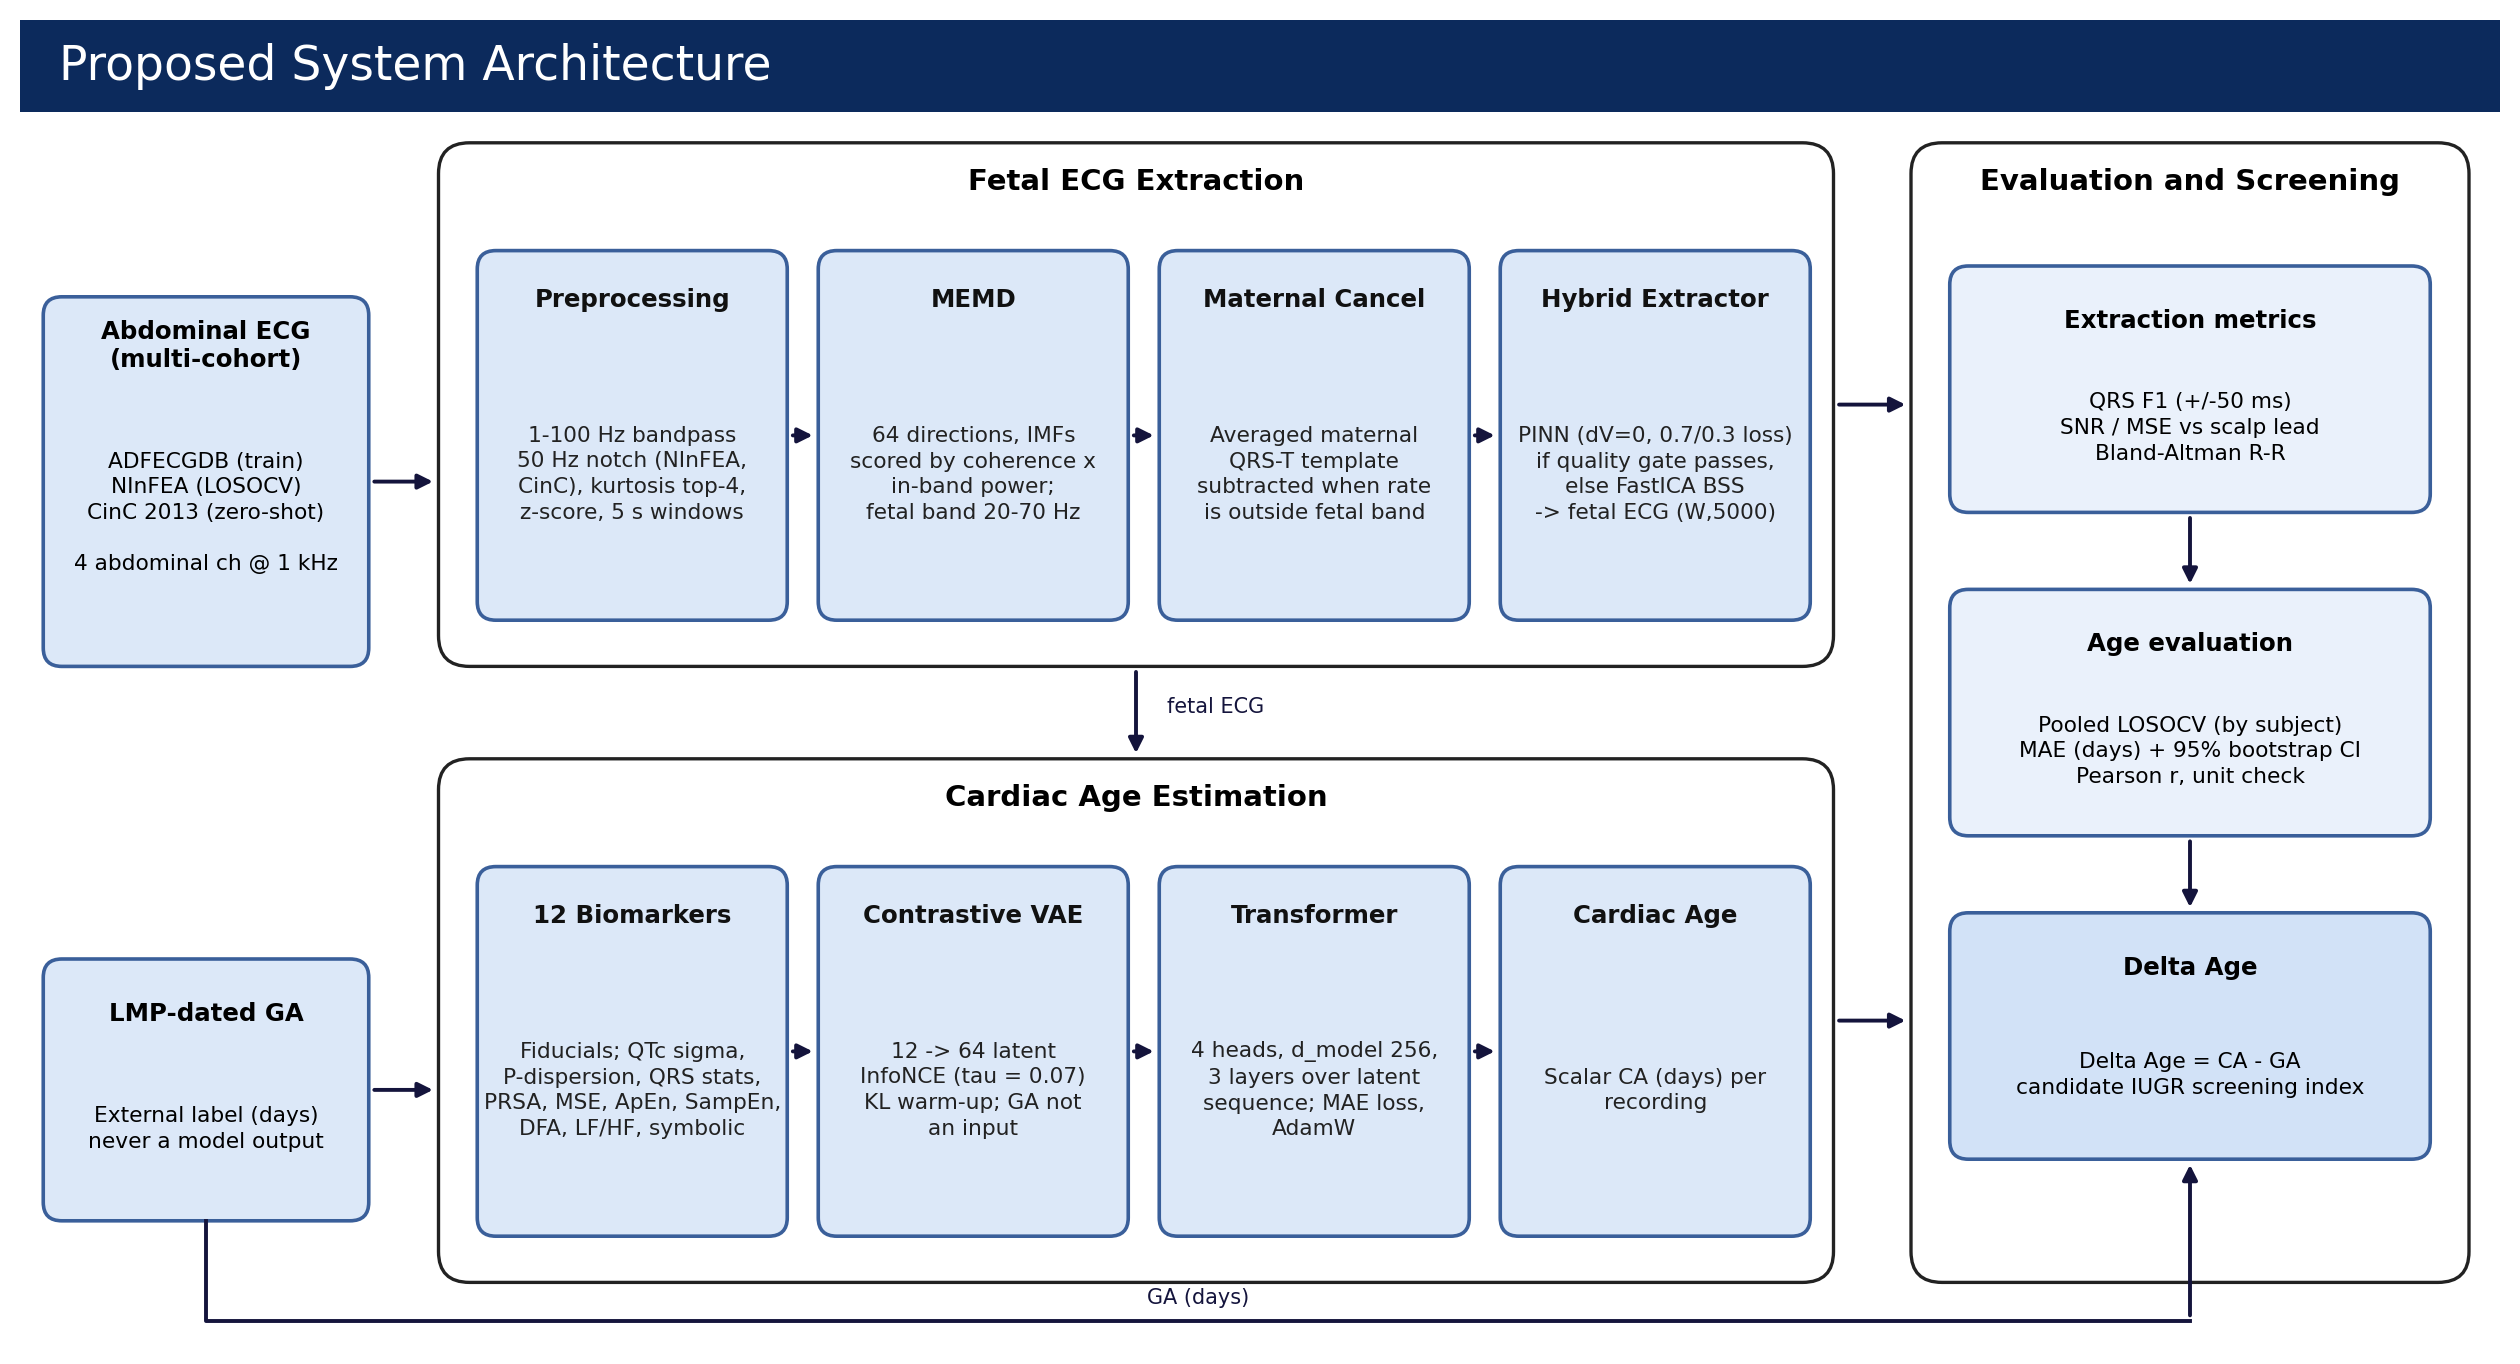
\includegraphics[width=0.92\textwidth]{figs/architecture_block.png}
\caption{Proposed pipeline: fetal ECG extraction (top), cardiac age estimation (bottom) and evaluation (right). GA is an external label and is never a model input or output.}
\label{fig:arch}
\end{figure*}

\subsection{Preprocessing}
Following~\cite{muthukumar2026icc}, signals are band-pass filtered (zero-phase Butterworth, 1--100~Hz), z-scored per channel per recording, and cut into non-overlapping 5000-sample (5~s) windows. A 50~Hz notch is applied to NInFEA and CinC 2013, where mains was measured to be prominent (13 of 25 CinC records), but not to ADFECGDB. For NInFEA the order is: filter at the native 2048~Hz rate, select the 4 highest-kurtosis abdominal channels (kurtosis computed after filtering, because raw drift inflates it), resample to 1000~Hz, normalise, window.

Fig.~\ref{fig:prep} shows raw and preprocessed signals with Welch spectra for ADFECGDB r08.

\begin{figure}[!t]
\centering
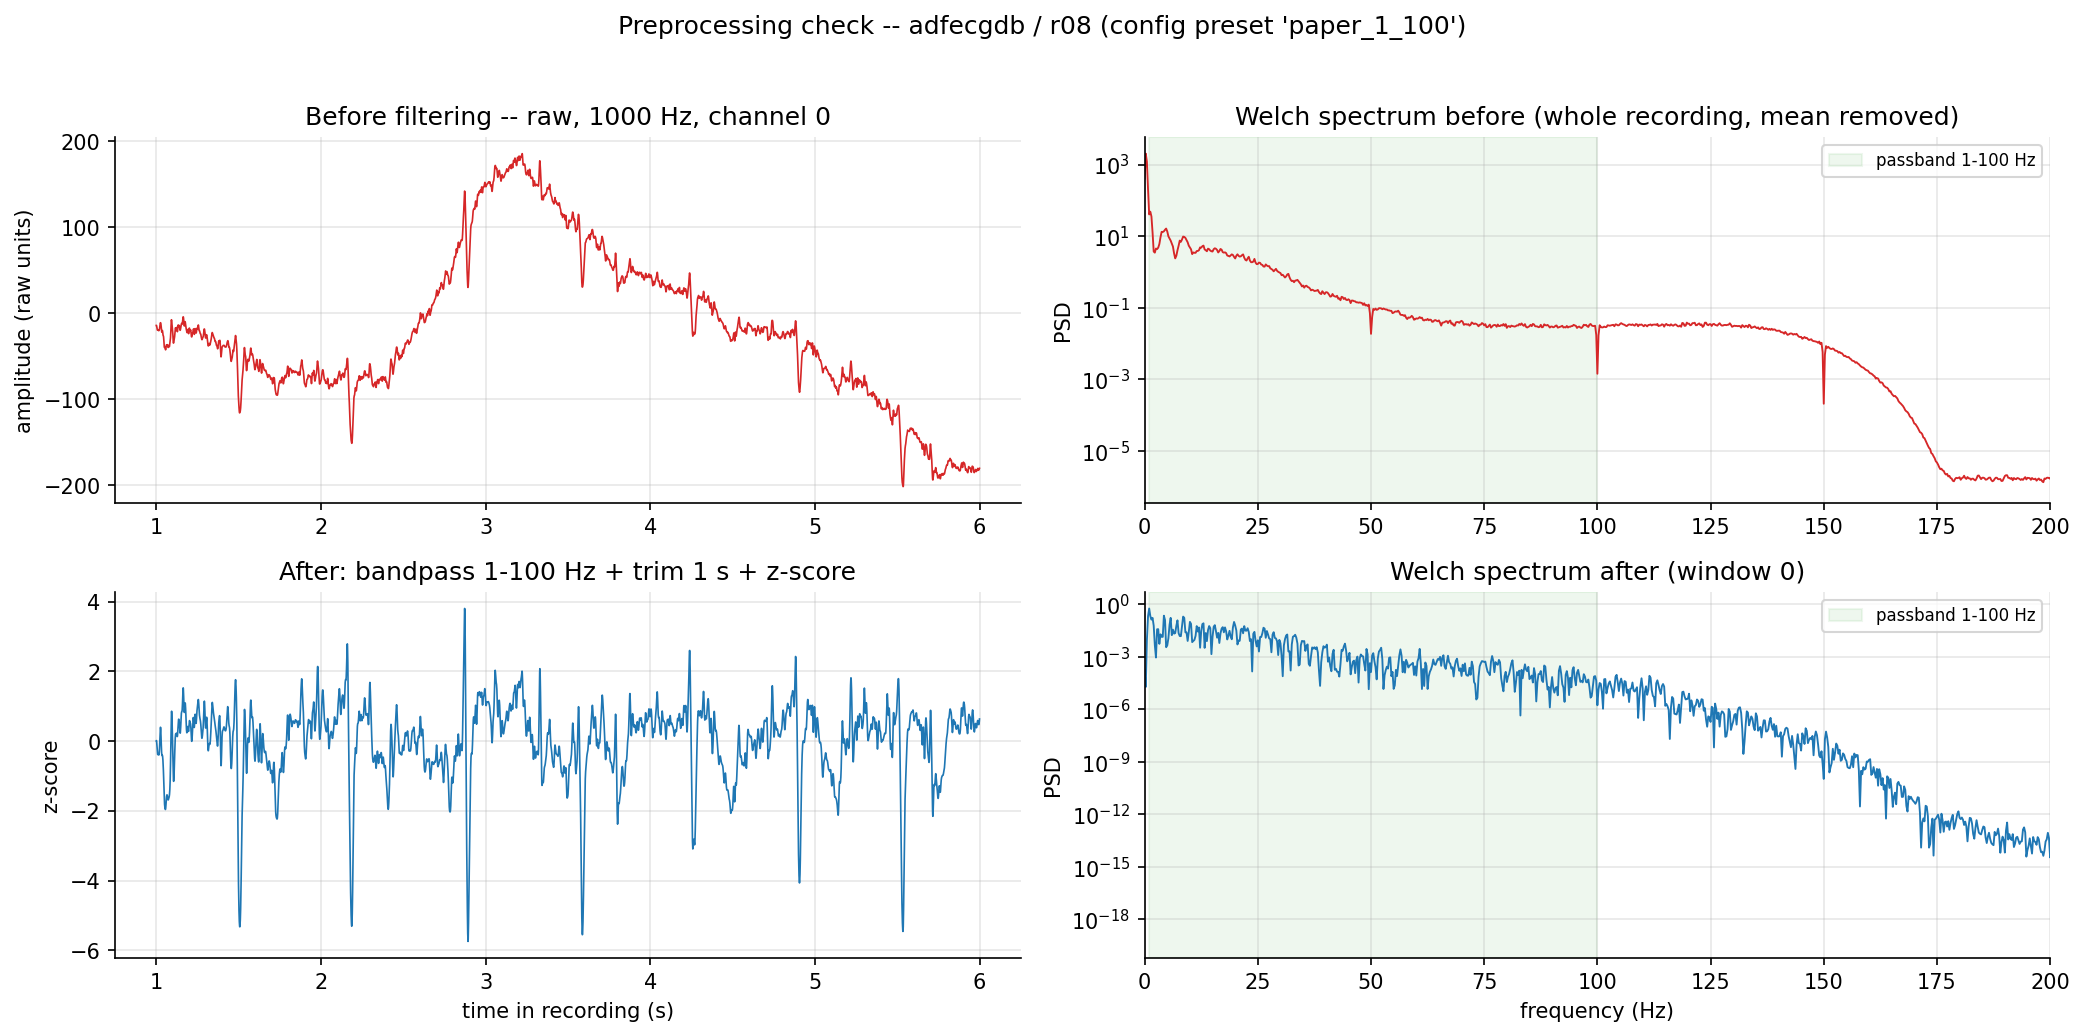
\includegraphics[width=\columnwidth]{figs/preprocessing_4ch.png}
\caption{ADFECGDB r08: raw versus preprocessed signal (1--100~Hz band-pass, 1~s trim, z-score) with Welch spectra before and after.}
\label{fig:prep}
\end{figure}

\subsection{Multivariate EMD}
Each window is decomposed by Hammersley-sequence MEMD~\cite{rehman2010} with 64 projection directions. IMFs are scored by spectral coherence times in-band power over the fetal band (20--70~Hz) and the selected IMFs are summed. The number of IMFs is data-determined (about 10--14). MEMD only removes drift, motion and muscle artefact; maternal--fetal separation is left to later stages. Results are cached per recording and window. Fig.~\ref{fig:memd} shows the per-IMF scores and the resulting fetal-band signal for ADFECGDB r01.

\begin{figure}[!t]
\centering
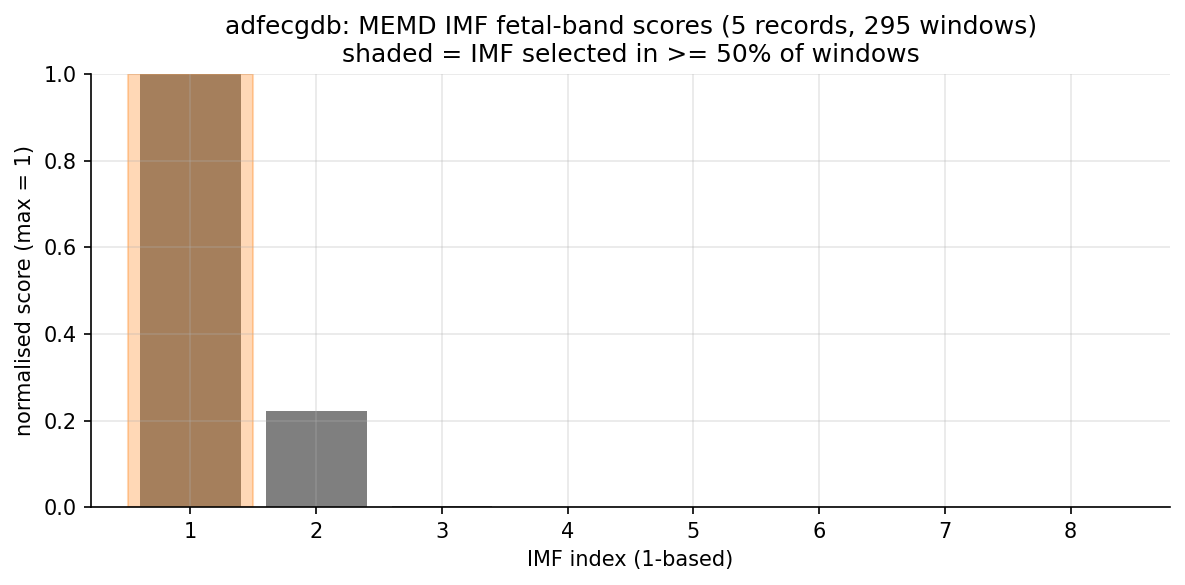
\includegraphics[width=\columnwidth]{figs/memd_fetal_band.png}
\caption{MEMD fetal-band extraction on ADFECGDB r01: spectral-correlation score per IMF, the maternal-dominant preprocessed signal, the fetal-band signal with artefacts removed, and the scalp ECG ground truth.}
\label{fig:memd}
\end{figure}

\subsection{Maternal cancellation}
An averaged maternal QRS-T template is subtracted from a window only when the detected rate falls outside the fetal band. This addresses a failure we measured directly: without it, ADFECGDB r04, r07 and r10 were extracted at the maternal rate (82--93~bpm).

\subsection{Physics-informed network}
The PINN~\cite{raissi2019} has five fully connected layers of 512 units (Tanh in layers 1--3; ReLU and dropout 0.2 in layers 4--5) and predicts a potential $V$. The Laplace constraint $\nabla^{2}V=0$ is enforced by double automatic differentiation at interior collocation points, with loss
\begin{equation}
\mathcal{L}=0.7\,\mathcal{L}_{\mathrm{data}}+0.3\,\mathcal{L}_{\mathrm{physics}}.
\end{equation}
The input is $[x,y,z,t,\mathrm{obs}_0,\ldots,\mathrm{obs}_3]$ (8-dimensional) and the fECG is read from the potential channel. This coordinate scheme is an assumption of ours, not a published specification, and it awaits supervisor sign-off; all PINN numbers below are marked with \pinn. The PINN is trained on ADFECGDB only and frozen thereafter. On ADFECGDB the potential read-out scored a QRS F1 of 0.519 against 0.443 for the residual read-out, suggesting that the constraint acts as a spatial denoiser rather than a maternal absorber.

\subsection{FastICA fallback and hybrid extractor}
FastICA~\cite{hyvarinen2000} is run on the four preprocessed channels. The fetal component is chosen without annotations: a rate within 110--160~bpm and the most regular rhythm. The \emph{hybrid} extractor uses, per window, the cancellation+PINN output if it passes the quality gate (rate 110--160~bpm, at least 5 beats, RR-artefact rate at most 25\%), and the FastICA output otherwise. A record is usable if at least half its windows pass.

\subsection{Biomarkers}
Fiducial points are detected on the extracted fECG and 12 features are computed: QTc $\sigma$, P-wave dispersion, QRS mean, variance and asymmetry, phase-rectified signal averaging (PRSA), multiscale entropy (MSE), approximate entropy, sample entropy, detrended fluctuation exponent $\alpha$, LF/HF ratio, and symbolic dynamics. Several entropy and scaling features are undefined on 5~s windows (mostly NaN), which matters in Section~VI-D.

\subsection{Contrastive VAE and transformer}
A contrastive VAE~\cite{kingma2014} maps the 12-feature window vector to a 64-dimensional latent with reconstruction, KL (with warm-up) and InfoNCE~\cite{oord2018} terms ($\tau=0.07$); positives are windows of the same subject or the same GA. GA is not an input. Inputs are standardised with training-set statistics. A transformer encoder~\cite{vaswani2017} (4 heads, $d_{\mathrm{model}}=256$, $d_k=64$, 3 layers, CLS pooling) takes each recording's sequence of latents and outputs a scalar CA, trained with an MAE loss and AdamW~\cite{loshchilov2019}.

\section{Experimental Protocol}
\textbf{Extraction.} Beat detection is scored by QRS F1 with a $\pm50$~ms tolerance against the reference QRS positions (ADFECGDB, CinC 2013). ADFECGDB is in-sample for the PINN; CinC 2013 is never trained on. NInFEA has no beat annotations, so we ported the dataset's Doppler-envelope extractor to the 60 pulsed-wave bitmaps and added peak detection (60/60 recordings, median 141~bpm, range 128--156~bpm). Doppler peaks lag the R wave by an unknown offset (estimated at about $-62$~ms with weak concentration), so for NInFEA we rely mainly on heart-rate agreement, which does not depend on the lag.

\textbf{SNR.} For a window of $T$ samples let $x$ be the preprocessed abdominal signal, $\hat f$ the extracted fetal ECG and $f_{\mathrm{ref}}$ the scalp reference, all z-scored. With
\begin{equation}
\mathrm{SNR}(s)=10\log_{10}\frac{\sum_n f_{\mathrm{ref}}[n]^2}{\sum_n (s[n]-f_{\mathrm{ref}}[n])^2},
\end{equation}
the improvement is $\Delta\mathrm{SNR}=\mathrm{SNR}(\hat f)-\mathrm{SNR}(x)$. Because the extractors are not trained to reproduce the reference amplitude, we also report a gain-matched SNR in which the best scalar gain (including sign) is applied to $\hat f$ per window. SNR is computed only on ADFECGDB, the sole cohort with a scalp lead.

\textbf{Age estimation.} CVAE and transformer are trained on ADFECGDB plus the NInFEA recordings that pass the gate, evaluated by pooled leave-one-subject-out cross-validation in which all recordings of a mother are held out together and the CVAE (and its imputation medians) is refitted inside every fold. With $N$ recordings, $\mathrm{MAE}=\frac1N\sum_i|GA_i-\widehat{CA}_i|$, $\mathrm{RMSE}=\sqrt{\frac1N\sum_i(GA_i-\widehat{CA}_i)^2}$, and $r=\mathrm{Corr}(GA,\widehat{CA})$. We report MAE in days with a 95\% bootstrap CI (1000 resamples, 2.5--97.5 percentile), Pearson $r$, and a predict-the-mean baseline; a unit-verification script checks days against weeks before any number is reported. Random seeds are fixed throughout.

\section{Results}
\subsection{Extraction on labelled cohorts}
Table~\ref{tab:f1} gives QRS F1. The hybrid is best on both cohorts; on CinC 2013, which is unseen by every trained component, the FastICA fallback alone (0.519) already beats the PINN-based arms, and the hybrid adds a further 0.023.

\begin{table}[!t]
\caption{QRS F1 ($\pm50$~ms). ADFECGDB is in-sample for the PINN. \pinn~PINN coordinate scheme pending sign-off.}
\label{tab:f1}
\centering
\small
\begin{tabular}{@{}lcc@{}}
\toprule
Method & ADFECGDB & CinC 2013 \\
\midrule
PINN\pinn & 0.510 & 0.377 \\
Cancellation + PINN\pinn & 0.630 & 0.440 \\
FastICA BSS & 0.557 & 0.519 \\
\textbf{Hybrid} & \textbf{0.637} & \textbf{0.542} \\
\bottomrule
\end{tabular}
\end{table}

Usable records (gate passed) rise with the hybrid from 2 to 5 of 5 on ADFECGDB (153 to 272 windows) and from 3 to 55 of 60 on NInFEA (19 to 265 windows). Fig.~\ref{fig:sep} shows a window on ADFECGDB r08 and Fig.~\ref{fig:ba} a Bland--Altman comparison of R--R intervals on CinC 2013.

\begin{figure}[!t]
\centering
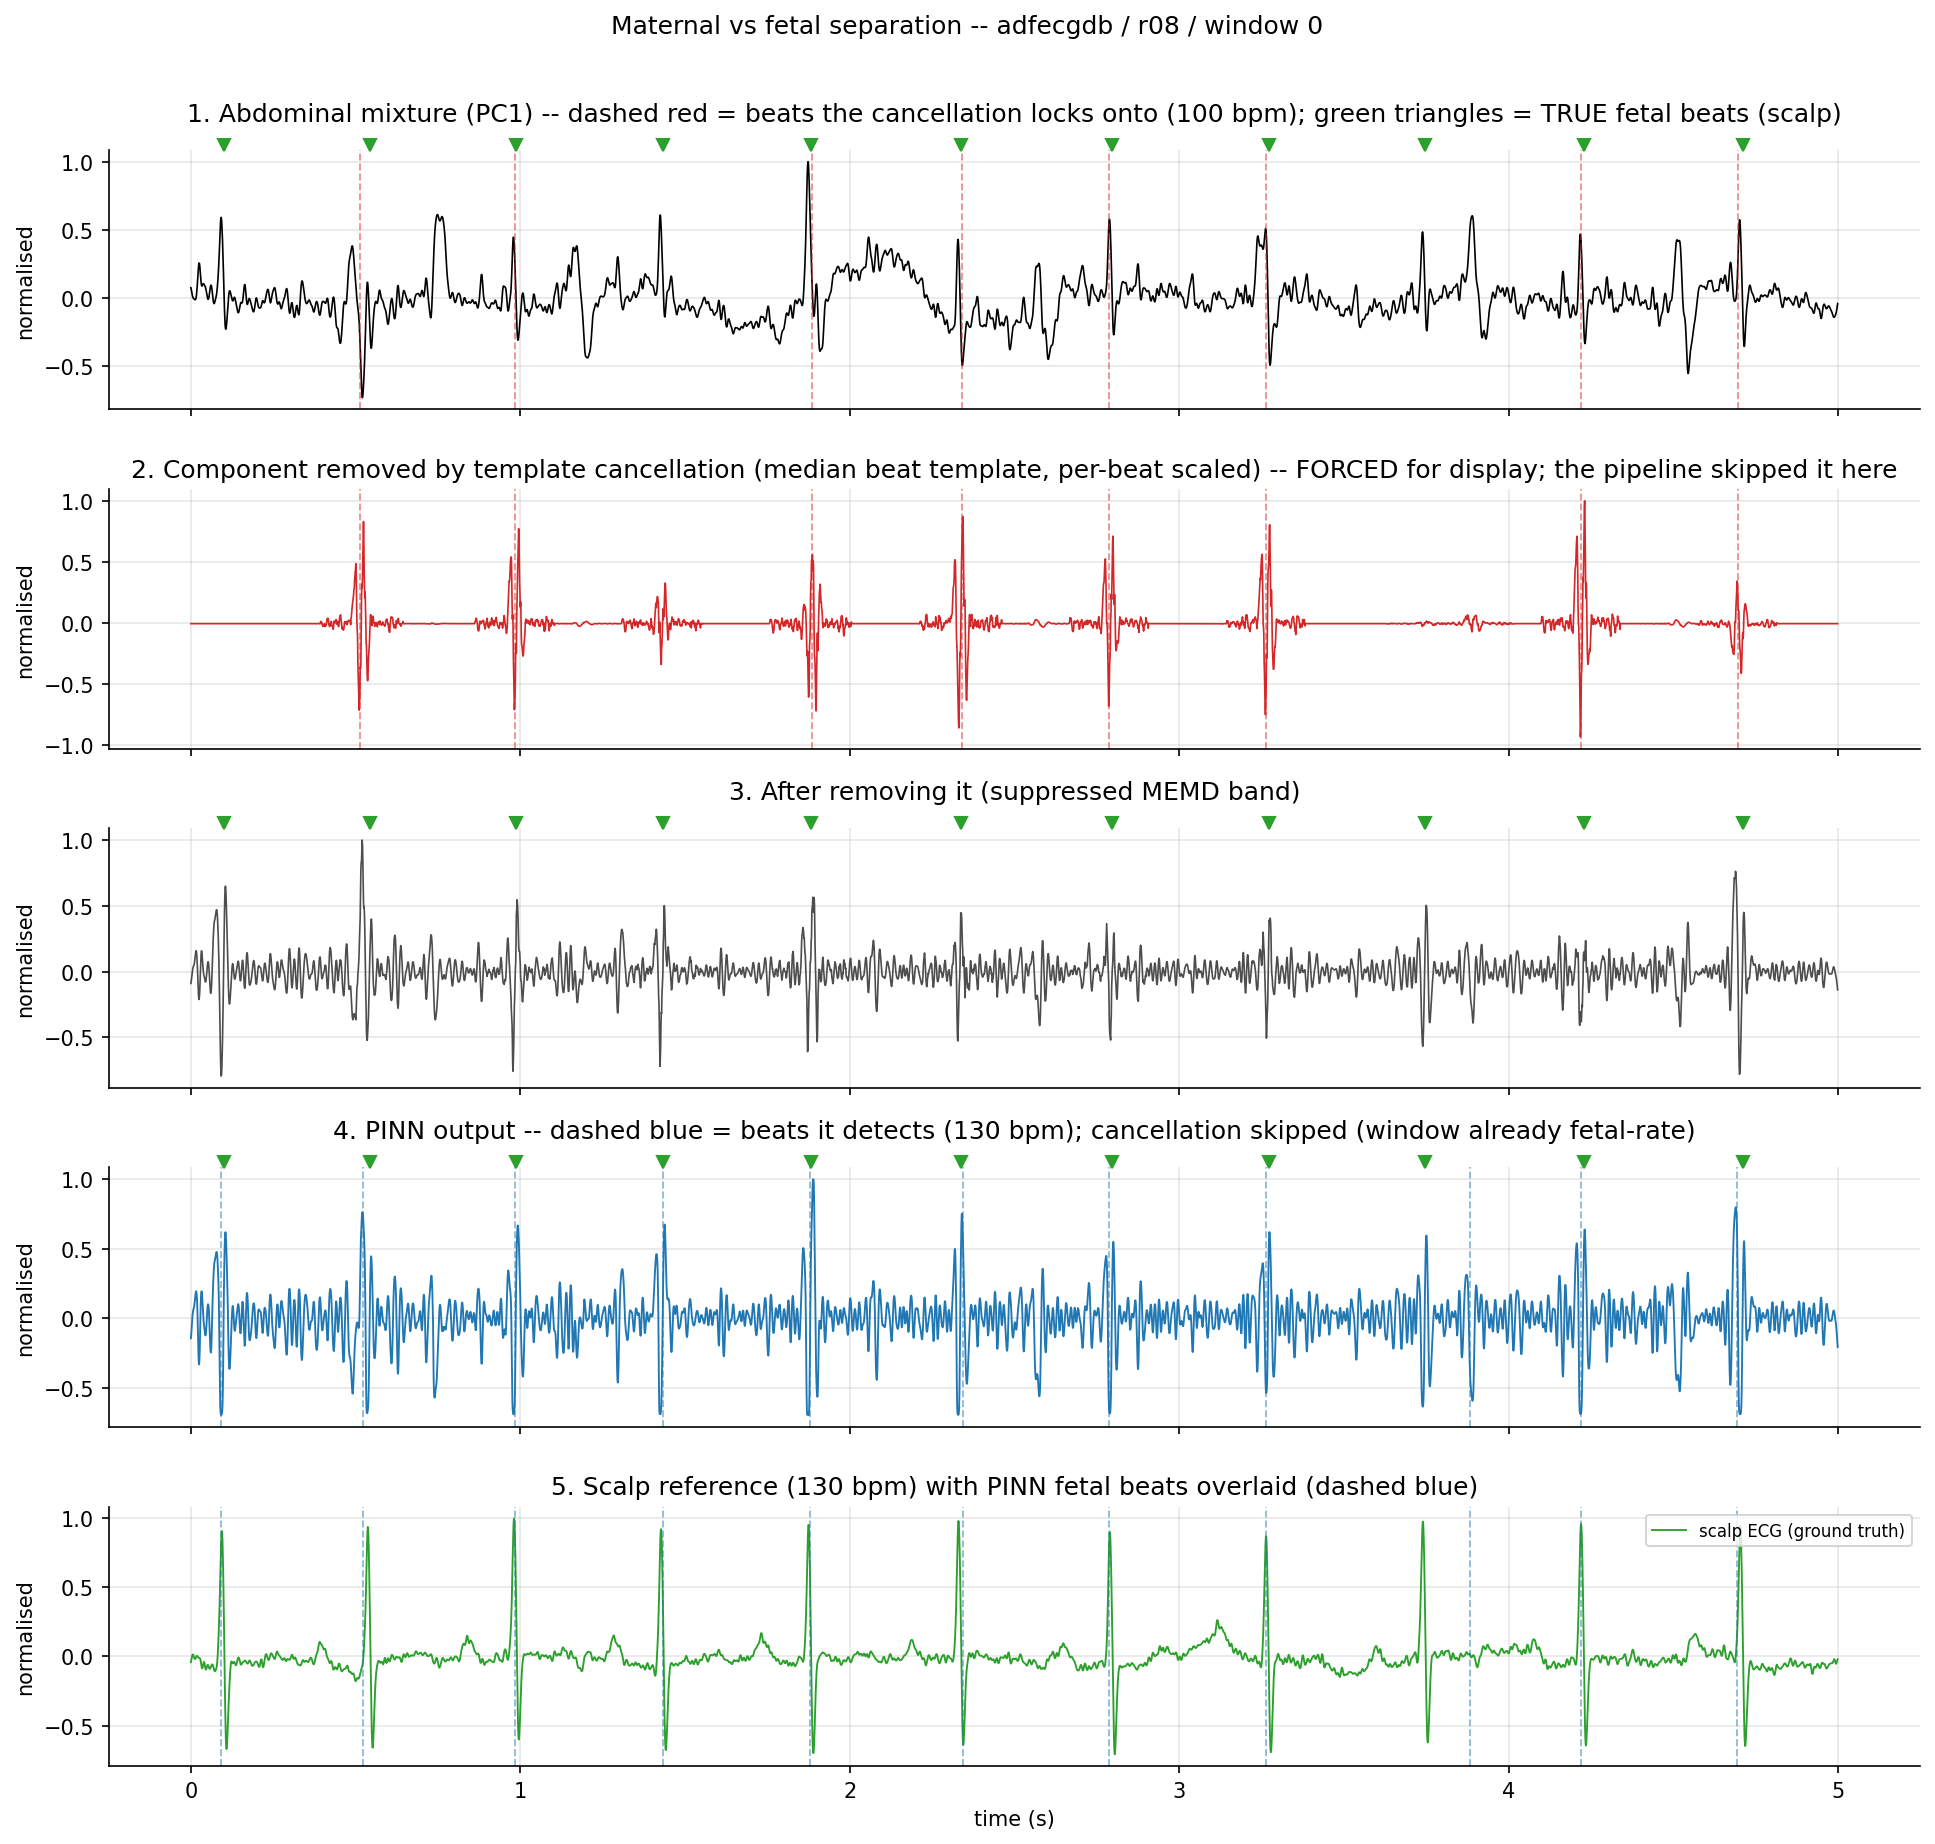
\includegraphics[width=\columnwidth]{figs/pinn_separation.png}
\caption{Extraction on ADFECGDB r08, window 0: abdominal mixture, template-cancelled component, PINN output and scalp reference with detected beats.}
\label{fig:sep}
\end{figure}

\begin{figure}[!t]
\centering
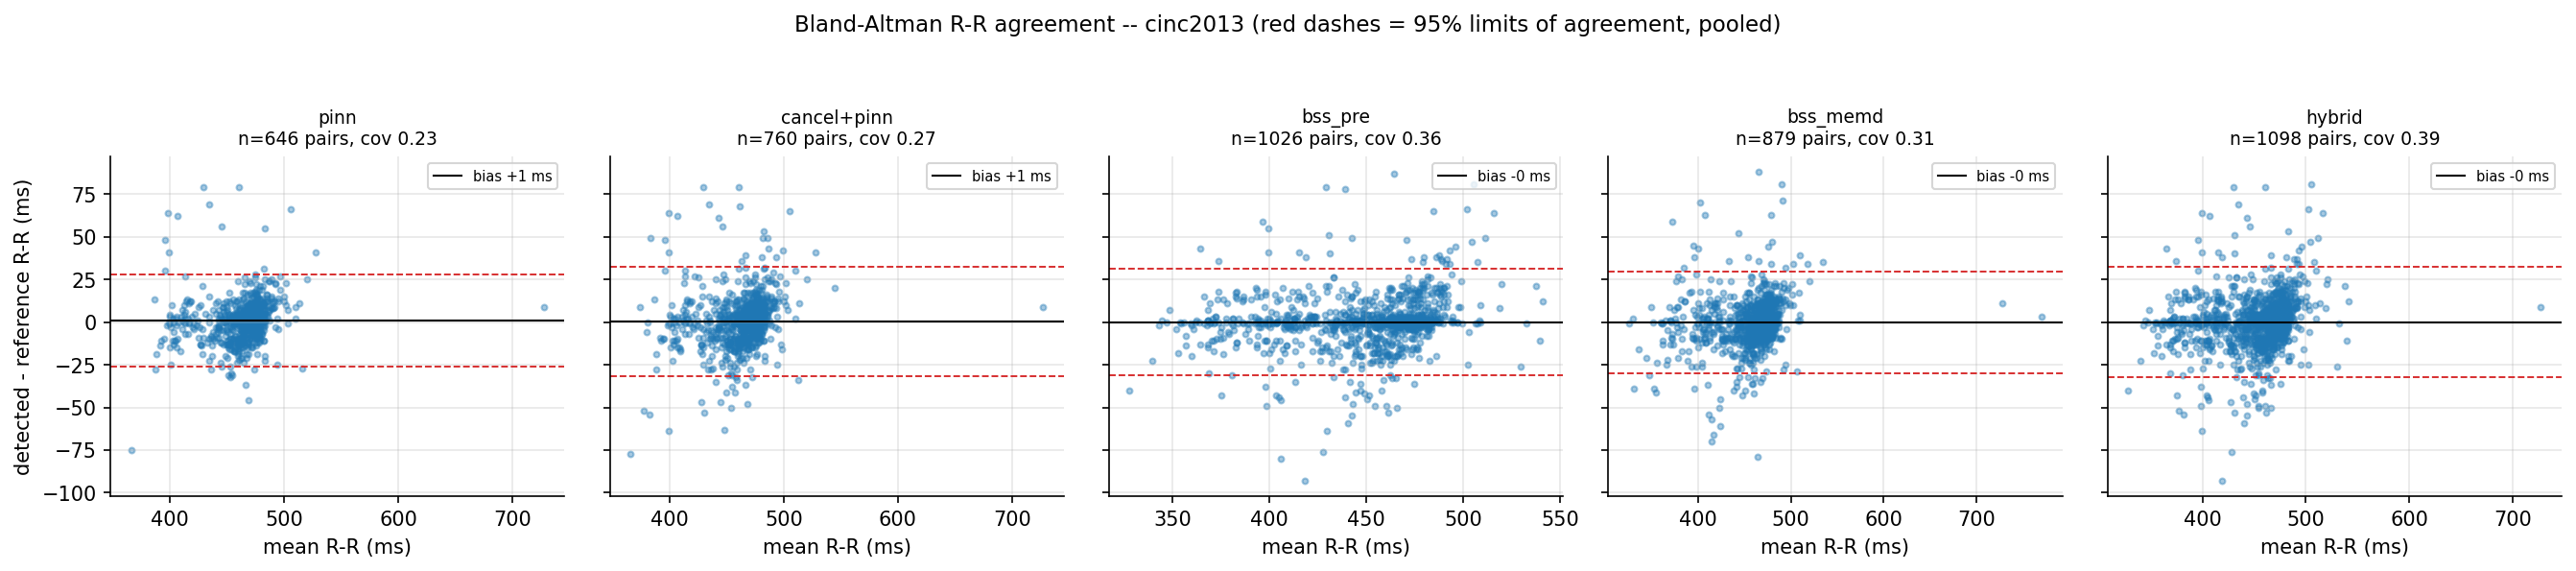
\includegraphics[width=\columnwidth]{figs/bland_altman_cinc2013.png}
\caption{Bland--Altman agreement of extracted and reference R--R intervals, CinC 2013.}
\label{fig:ba}
\end{figure}

\subsection{NInFEA against Doppler}
On 315 windows from 60 recordings, the PINN-based arms lock onto the maternal rhythm (Table~\ref{tab:doppler}). The beat F1 against Doppler is 0.23 for both BSS and hybrid at $\pm50$~ms (0.43--0.44 at $\pm100$~ms) against 0.17 and 0.14 for the PINN arms; it is approximate because of the unknown lag. The quality gate keeps 98\% of right-rate windows, but only 63\% of the windows it keeps have the right rate, so a high gate-pass rate overstates correctness.

\begin{table}[!t]
\caption{NInFEA heart-rate agreement with Doppler (315 windows). \pinn~pending sign-off.}
\label{tab:doppler}
\centering
\small
\begin{tabular}{@{}lcc@{}}
\toprule
Method & Within 10 bpm & Median error (bpm) \\
\midrule
PINN\pinn & 2\% & 53 \\
Cancellation + PINN\pinn & 5\% & 59 \\
FastICA BSS & 52\% & 10 \\
\textbf{Hybrid} & \textbf{54\%} & \textbf{9} \\
\bottomrule
\end{tabular}
\end{table}

An experimental PINN trained on ADFECGDB plus NInFEA (split by mother) did not help: NInFEA gate pass 4.8\% against 6.0\%, CinC 2013 F1 0.380 against 0.377 (2 folds, 200 epochs)\pinn. The failure is maternal lock, not a lack of PINN training data, so the ADFECGDB-only PINN remains the default.

\subsection{SNR against the scalp lead}
On ADFECGDB, gain-matched SNR over all windows is 0.43~dB (PINN\pinn), 0.44 (cancellation+PINN\pinn), 0.41 (BSS) and 0.45 (hybrid); the best raw abdominal channel gives 0.33~dB. In the unit-gain, sign-aligned form used in~\cite{muthukumar2026icc} the values are about $-1.7$~dB with MSE near 1.55. Clean records r01 and r08 reach roughly 0.9--1.2~dB while r04, r07 and r10 stay near 0, and allowing a $\pm40$~ms shift raises the mean only to about 0.6~dB. The abdominal fetal waveform differs in shape from the scalp lead, so sample-wise SNR is low even when beat detection is good (F1 above 0.9 on r01 and r08). It does not separate the methods and is not comparable with the 14.4~dB reported in~\cite{muthukumar2026icc}, whose network was trained to reproduce the scalp signal. Beat-timing metrics are the informative ones here.

\subsection{Biomarkers, CVAE and age estimation}
\emph{CVAE.} On held-out data (537 windows, 44 subjects), standardising the inputs changed the median held-out per-feature $R^{2}$ from $-0.01$ to 0.86, the number of features beating the training mean from 3/11 to 11/11, and active latent dimensions from 19--39 to 64/64. Same-subject retrieval is 0.14 (chance 0.06, raw features 0.15). Because the latent (64) is larger than the input (12), good reconstruction shows the autoencoder works, not that the latent is informative: kNN GA prediction over 39 NInFEA mothers has MAE 12.3~d (latent), 11.1~d (raw features) and 11.4~d (predict the mean).

\emph{Is there an age signal?} Within NInFEA (GA 147--194~d, 6.7 weeks) the Doppler fetal heart rate has Spearman $\rho=-0.07$ against GA (60 recordings), and none of the 12 features is significant after Bonferroni correction. Keeping only windows whose extracted rate matches the Doppler rate (166 windows, 51 recordings) does not change this: the strongest feature, symbolic dynamics, has $\rho=-0.25$ ($p=0.08$). With about 50 recordings only $|\rho|\gtrsim0.4$ is detectable, so weak effects are not excluded, but they would be too weak to support a predictor. MSE, SampEn, DFA and PRSA are mostly undefined on 5~s windows and could not be tested properly.

\emph{Transformer.} Table~\ref{tab:age} gives NInFEA-only strict leave-one-mother-out results. The model is worse than predicting the cohort mean and its predictions (150--275~d, s.d.\ 25) are far more spread than the true ages (s.d.\ about 15), i.e.\ it fits noise.

\begin{table}[!t]
\caption{Age estimation within NInFEA (59 recordings with features), leave-one-mother-out.}
\label{tab:age}
\centering
\small
\begin{tabular}{@{}lcc@{}}
\toprule
Model & MAE (days) & within-cohort $r$ \\
\midrule
Predict the NInFEA mean & 12.5 & -- \\
CVAE + transformer & 22.6 & $-0.02$ \\
\bottomrule
\end{tabular}
\end{table}

The pooled analysis that adds ADFECGDB yields a higher pooled correlation ($r=0.56$), but this arises from separating the two cohorts (21--27 against 38--41 weeks), and the ADFECGDB GA values used there were random placeholders. We therefore do not report pooled MAE as a result.

\section{Discussion and Limitations}
\textbf{The ageing claim is not supported by the current data.} The negative result has plausible causes that we cannot yet separate: (i) NInFEA spans only 6.7 weeks, so true effects may be small relative to between-fetus variation; (ii) 5~s windows are too short for the slowly varying dynamic features; (iii) no cohort covers 28--37 weeks, so a model trained on 38--41 weeks cannot be tested on 21--27 weeks without extrapolation; (iv) NInFEA windows are mostly FastICA output (only about 6\% come from the PINN) and about half have the correct heart rate.

\textbf{ADFECGDB gestational ages.} PhysioNet gives only the range 38--41 weeks. Until the five per-record LMP-dated values are obtained, every analysis involving ADFECGDB GA is a pipeline check, and the ageing part of the framework has no external-validation cohort (CinC 2013 has no GA).

\textbf{Evaluation caveats.} The PINN is in-sample on ADFECGDB; NInFEA GA and the recording-to-mother table were taken from the dataset paper via a summarising tool and have not been checked against the published tables; the Doppler lag is estimated, not known; NInFEA is used for training the CVAE and transformer, so it is not a zero-shot set for those stages; and the PINN input-coordinate scheme is our assumption.

\textbf{Clinical scope.} $\Delta\mathrm{Age}$ as an IUGR index is a hypothesis. Nothing here evaluates it against growth-restricted fetuses.

\section{Conclusion}
A hybrid PINN/FastICA extractor with a quality gate recovers fetal rhythm markedly better than the PINN alone on cohorts it was not trained on, and makes 55 of 60 NInFEA recordings usable. The downstream cardiac-age model, however, shows no age information within the 21--27 week range and does not beat a predict-the-mean baseline. Future work needs real per-record ADFECGDB gestational ages, data spanning more of pregnancy, per-recording rather than per-window dynamic features, and sign-off of the PINN coordinate scheme before the age claim can be tested.

\section*{Acknowledgment}
\todo{acknowledgements}

\bibliographystyle{IEEEtran}
\bibliography{references}

\end{document}
